\documentclass[a4paper,12pt]{article}
\usepackage{graphicx}
\usepackage{tikz}
\usepackage{geometry}
\usepackage{textpos}
\usepackage[T1]{fontenc}
\usepackage[polish]{babel}
\usepackage[utf8]{inputenc}

\geometry{left=2cm,right=2cm,top=2cm,bottom=2cm}

\usepackage{helvet}
\renewcommand{\familydefault}{\sfdefault}

\usepackage{fancyhdr}
\pagestyle{fancy}
\fancyhf{}
\fancyfoot[R]{- \thepage/\pageref{LastPage} -}
\renewcommand{\headrulewidth}{0pt}
\usepackage{lastpage}
\usepackage{float}
\usepackage{datetime}
\usepackage{booktabs}


\newdateformat{mydate}{\THEYEAR-\twodigit{\THEMONTH}-\twodigit{\THEDAY}}
\graphicspath{{../SKRYPTY/FIG/}}

% %%%%%%%%%%%%%%%%%%%%%%%%%%%%%%%%%%%%%%%%%%%%%%%%%%%%%%%%%%

\newcommand{\tematZadania}{<Temat zadania>}
\newcommand{\Name}{\\Daniel Kotliński \\ Sklorz Konrad \\ Maciej Krupinski \\ Aleksander Łokieć \\ RAfał Mikołajczak}

%%%%%%%%%%%%%%%%%%%%%%%%%%%%%%%%%%%%%%%%%%%%%%%%%%%%%%%%%%%%

\begin{document}

\begin{tikzpicture}[remember picture, overlay]
    \draw[thick] (current page.north west) ++(0.35\paperwidth,-0.1\paperheight) -- ++(0,-0.7\paperheight);
\end{tikzpicture}

\begin{textblock*}{0.24\textwidth}(.6cm, 1cm)
    \begin{flushright}
    \large
    \textbf{
        Katedra Podstaw Konstrukcji Maszyn \\[1cm]
        Wydział Mechaniczny Technologiczny \\[1cm]
        Politechnika Śląska
    }
    \end{flushright}
\end{textblock*}

\begin{textblock*}{0.65\textwidth}(0.30\paperwidth, 5cm)
    \begin{flushleft}
        \Huge \textbf{Projektowanie \\Systemów \\ Diagnostycznych \\[1.5cm]}
        \LARGE \textbf{Raport końcowy} \\[1cm] 
        \normalsize \textbf{Rok akademicki:} 2024/25\\[.6cm]
        \textbf{Temat zadania:} \tematZadania\\[.6cm]
        \textbf{Studenci w sekcji:} \Name\\[.6cm]
        \textbf{Kierunek:} AiRP\\[.6cm]
        \textbf{Grupa:} AB5\\ [.6cm]
        \textbf{Data opracowania:} \mydate\today\\ 
    \end{flushleft}
\end{textblock*}

\begin{textblock*}{\textwidth}(0cm, 25.6cm)
    \begin{center}
        \color{gray}
        \small KPKM, MT, PolSl, Gliwice
    \end{center}
\end{textblock*}

\renewcommand{\familydefault}{\rmdefault}
\newpage


\section{Opis zadania projektowego}

\section{Opis diagnozowanego obiektu}


\section{Analiza dostępnych zmiennych procesowych}


\subsection{Wykresy zmiennych procesowych dla stanu pełnej zdatności oraz stanów z uszkodzeniami}

\subsubsection{Wykrycie przytkania}

Wykrycie przytkania na podstawie spadku przepływu w rurze. Na rys. \ref{fig:zatkanie1} przedsatwiono moment zatkania w 80\%. Widać, że mimo pełnego wysterowania pompy, nie duało się zrealizować rządanego przepływu.

Dla kontrastu na rys. \ref{fig:zatkanie2} przedstawiono moment zatkania w 40\%. Widać, że pomimo zatkania, udało się zrealizować rządaną wartość przepływu co utrudnia wykrycie tak małego zatkania.

\begin{figure}[H]
        \centering
        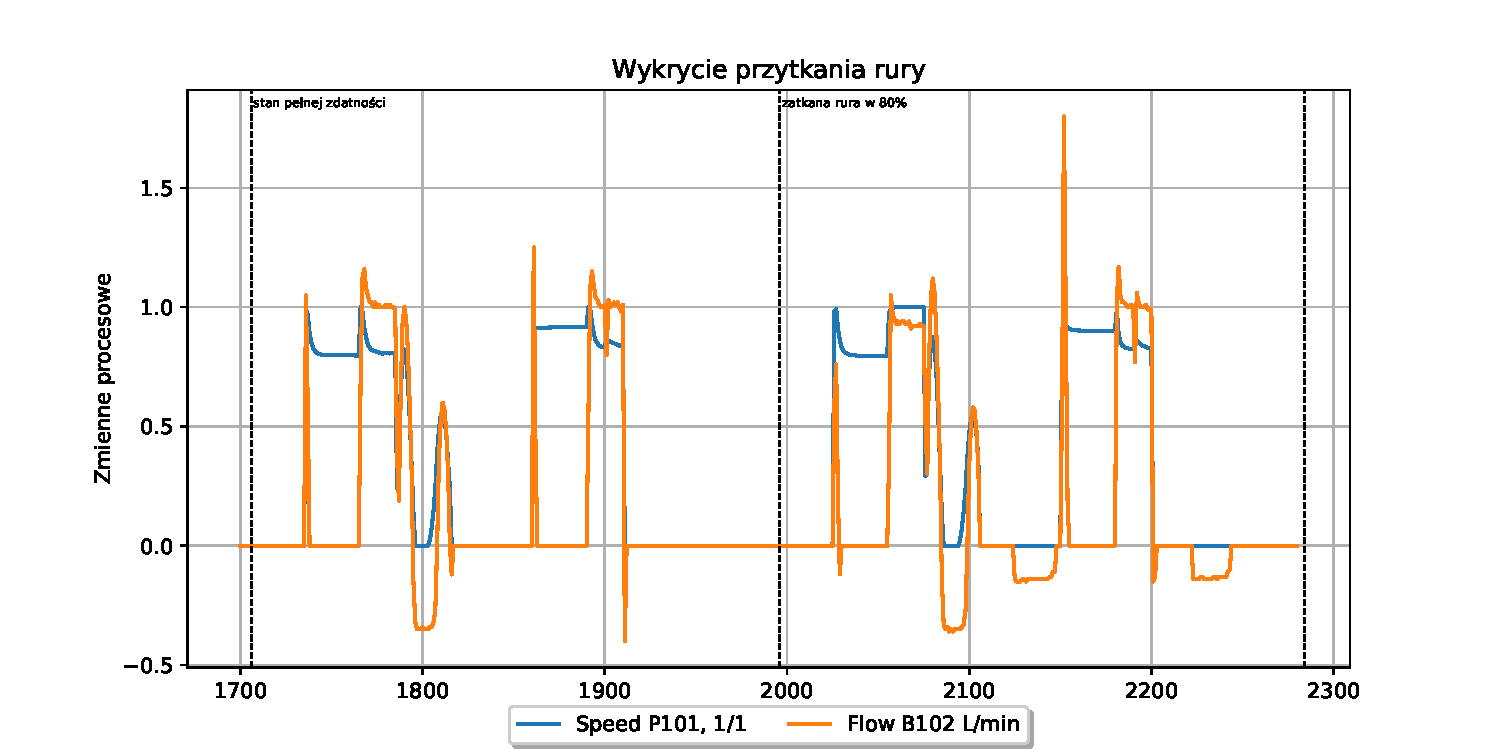
\includegraphics[width=0.8\textwidth]{clogging_detection_1700_2280.pdf}
        \caption{Test zatkania rury w 80\%}
        \label{fig:zatkanie1}
\end{figure}

\begin{figure}[H]
        \centering
        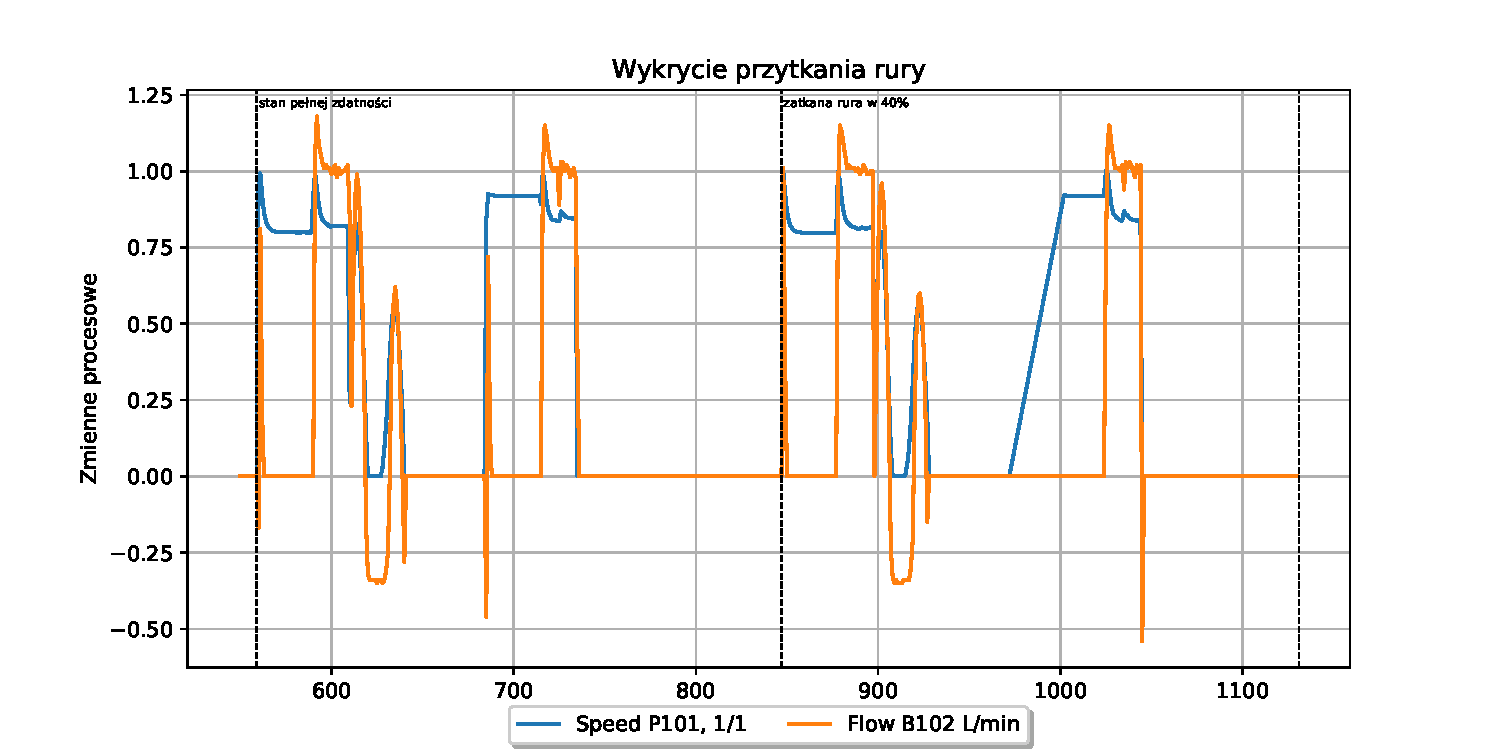
\includegraphics[width=0.8\textwidth]{clogging_detection_550_1130}
        \caption{Test zatkania rury w 40\%}
        \label{fig:zatkanie2}
\end{figure}


\subsubsection{Wykrycie cyberataku}
Na rys. \ref{fig:atak} przedstawiono moment cyberataku. Widać, że w momencie ataku, przepływ w rurze stał się niestabilny (duży RMS).

\begin{figure}[H]
        \centering
        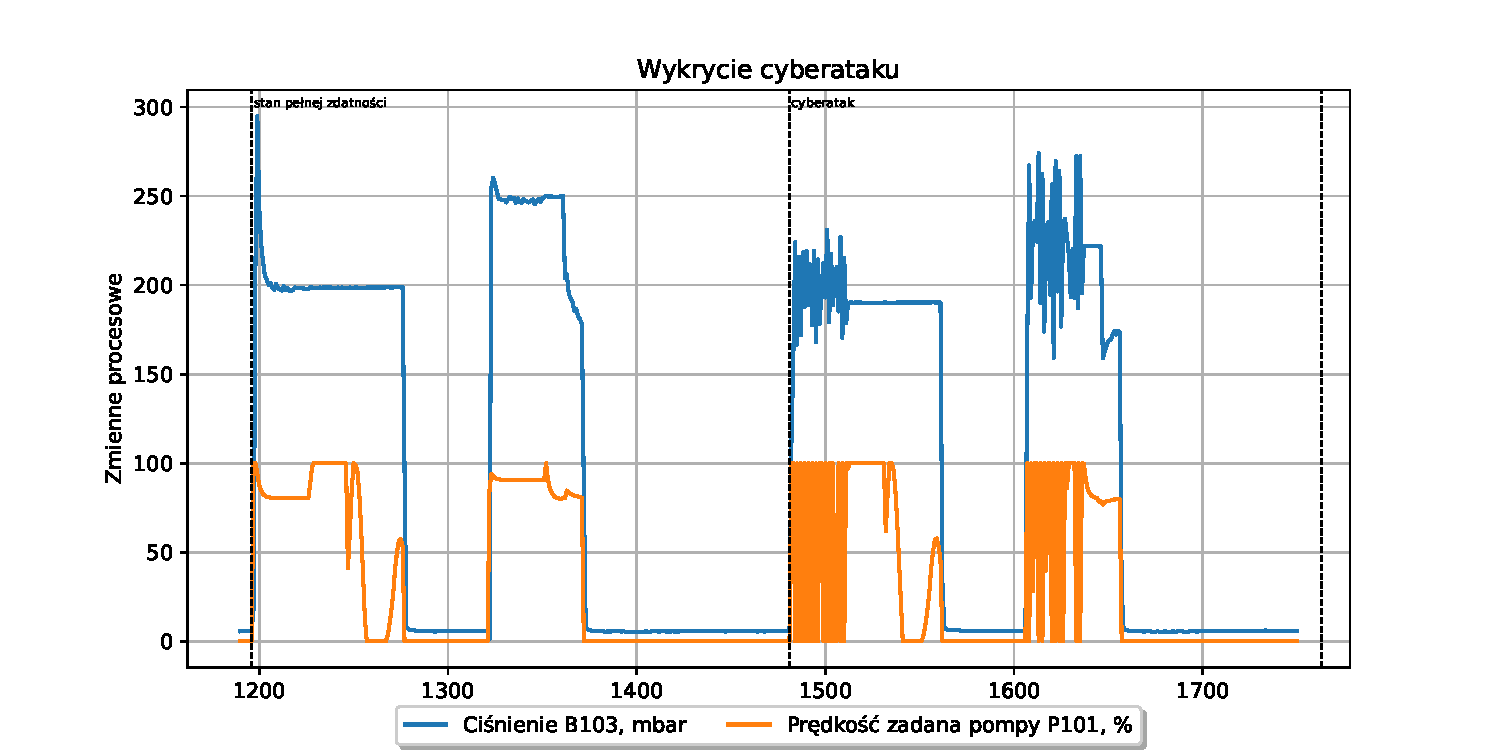
\includegraphics[width=0.8\textwidth]{attack_detection_1190_1750.pdf}
        \caption{Test cyberataku}
        \label{fig:atak}
\end{figure}

\subsubsection{Wykrycie wycieku}

Na rys. \ref{fig:wyciek1} przedstawiono moment wycieku. Porównano poziomy w zbiornikach oraz ich sumę (zbiorniki miały prawdopodobnie to samo pole przekroju). Widać, że w momentach wycieku suma poziomów nagle malała. Na rys. \ref{fig:wyciek2} przedsatwiono szerszy okres na którym wida cpowtarzalność zjawiska.

\begin{figure}[H]
        \centering
        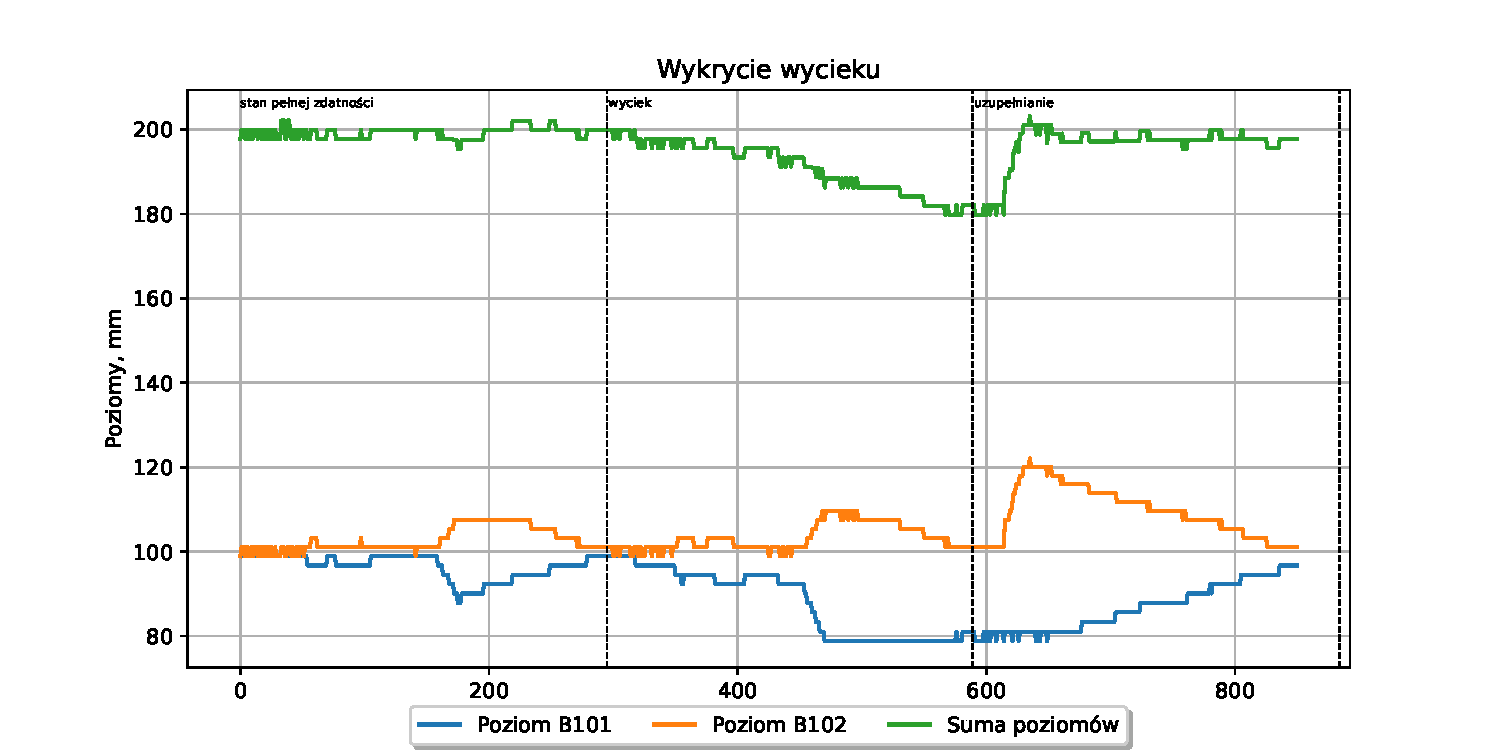
\includegraphics[width=0.8\textwidth]{leak_detection_0_850}
        \caption{Test wycieku}
        \label{fig:wyciek1}
\end{figure}

\begin{figure}[H]
        \centering
        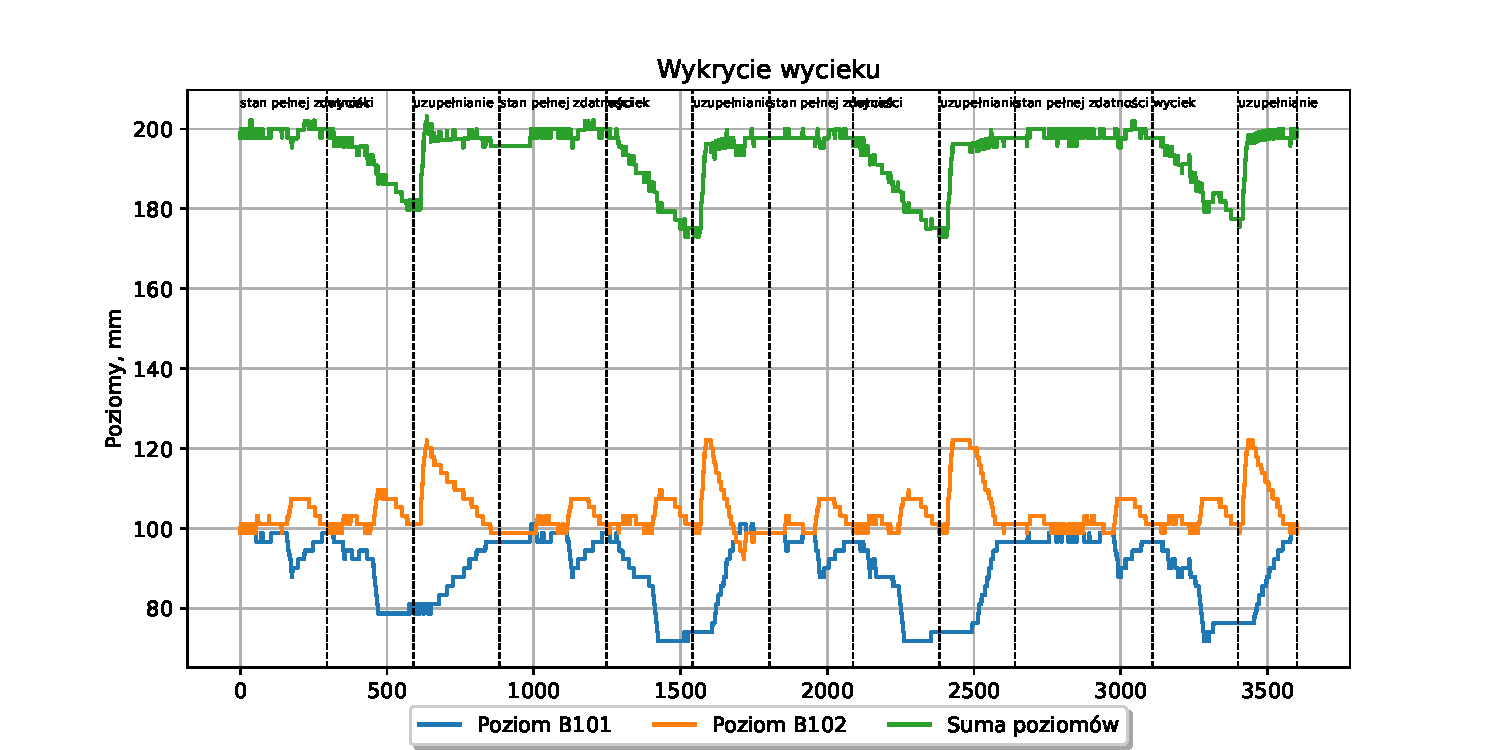
\includegraphics[width=0.8\textwidth]{leak_detection_-inf_inf}
        \caption{Test wycieku}
        \label{fig:wyciek2}
\end{figure}

\subsubsection{Wykrycie błędu operatora}
Na rys. \ref{fig:error} przedstawiono moment błędu operatora. Widać, że w odpowiednich fazach zadane ciśnienie w zbiorniku nie jest utrzymywane.

\begin{figure}[H]
        \centering
        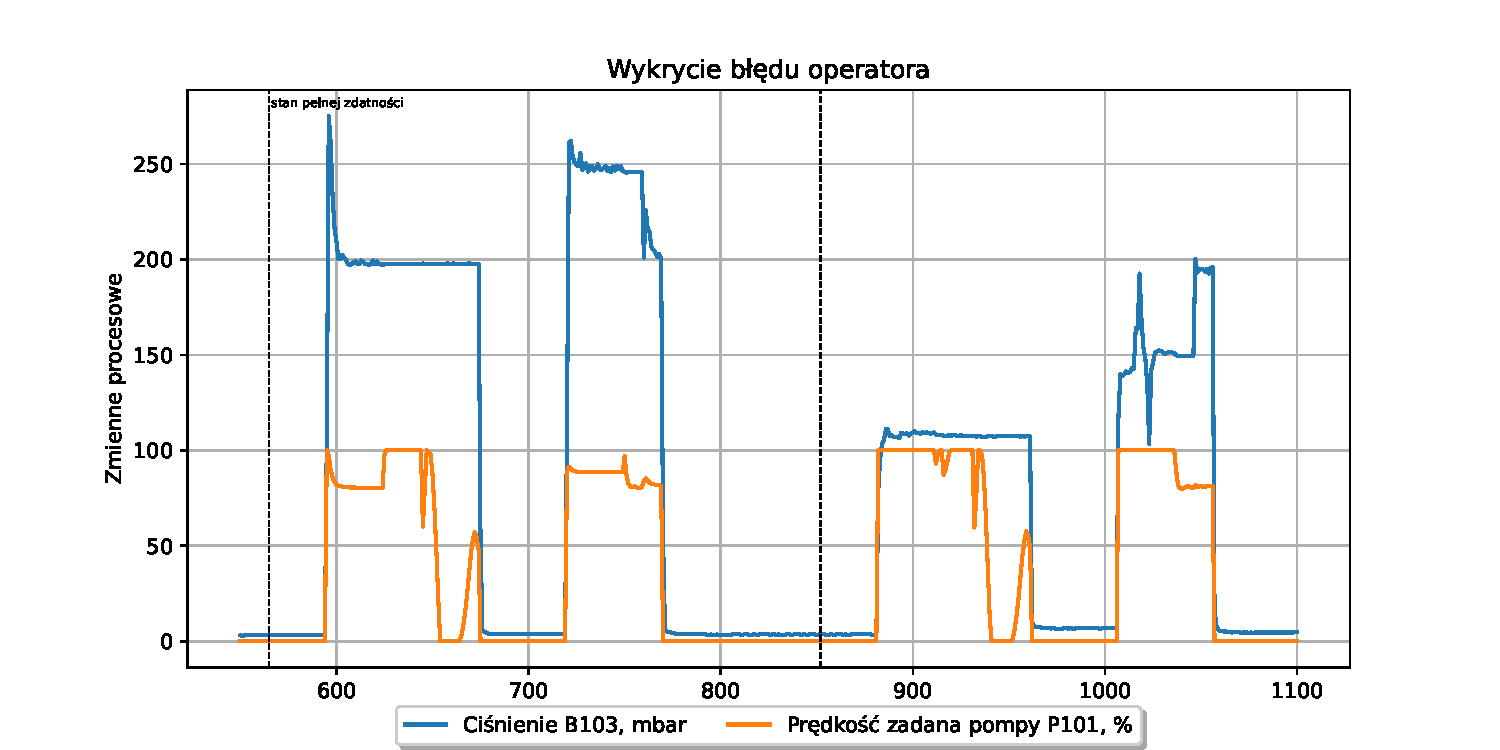
\includegraphics[width=0.8\textwidth]{error_detection_550_1100}
        \caption{Test błędu operatora}
        \label{fig:error}
\end{figure}

\subsection{Opis symptomów poszczególnych stanów}


\section{Testy diagnostyczne bazujące na diagnozowaniu bezpośrednim}

Zaimplementowano kilka metod służących do deteklcji i izolacji konkretnych stanów. Przykłady przedstawiono poniżej.

\subsection{Wykrycie wycieku}

W celu wykrycia wyceku sprawdzana jest suma poziomów w dwóch zbiornikach. W przypadku wycieku suma ta nagle maleje. Przed testem suma poziomów jest ustawiana. Wybrano arbitralną sume poziomów dla którego uznaje się że wystąpił wyciek. Wartość ta wynosi 190cm. Na rys. \ref{fig:wyciek1} przedstawiono działanie testu diagnostycznego dla przebiegu z awariami. Jak widać, wszystkie wycieki zostały wykryte, oraz nie wystąpiły fałszywe alarmy.

\begin{figure}[H]
        \centering
        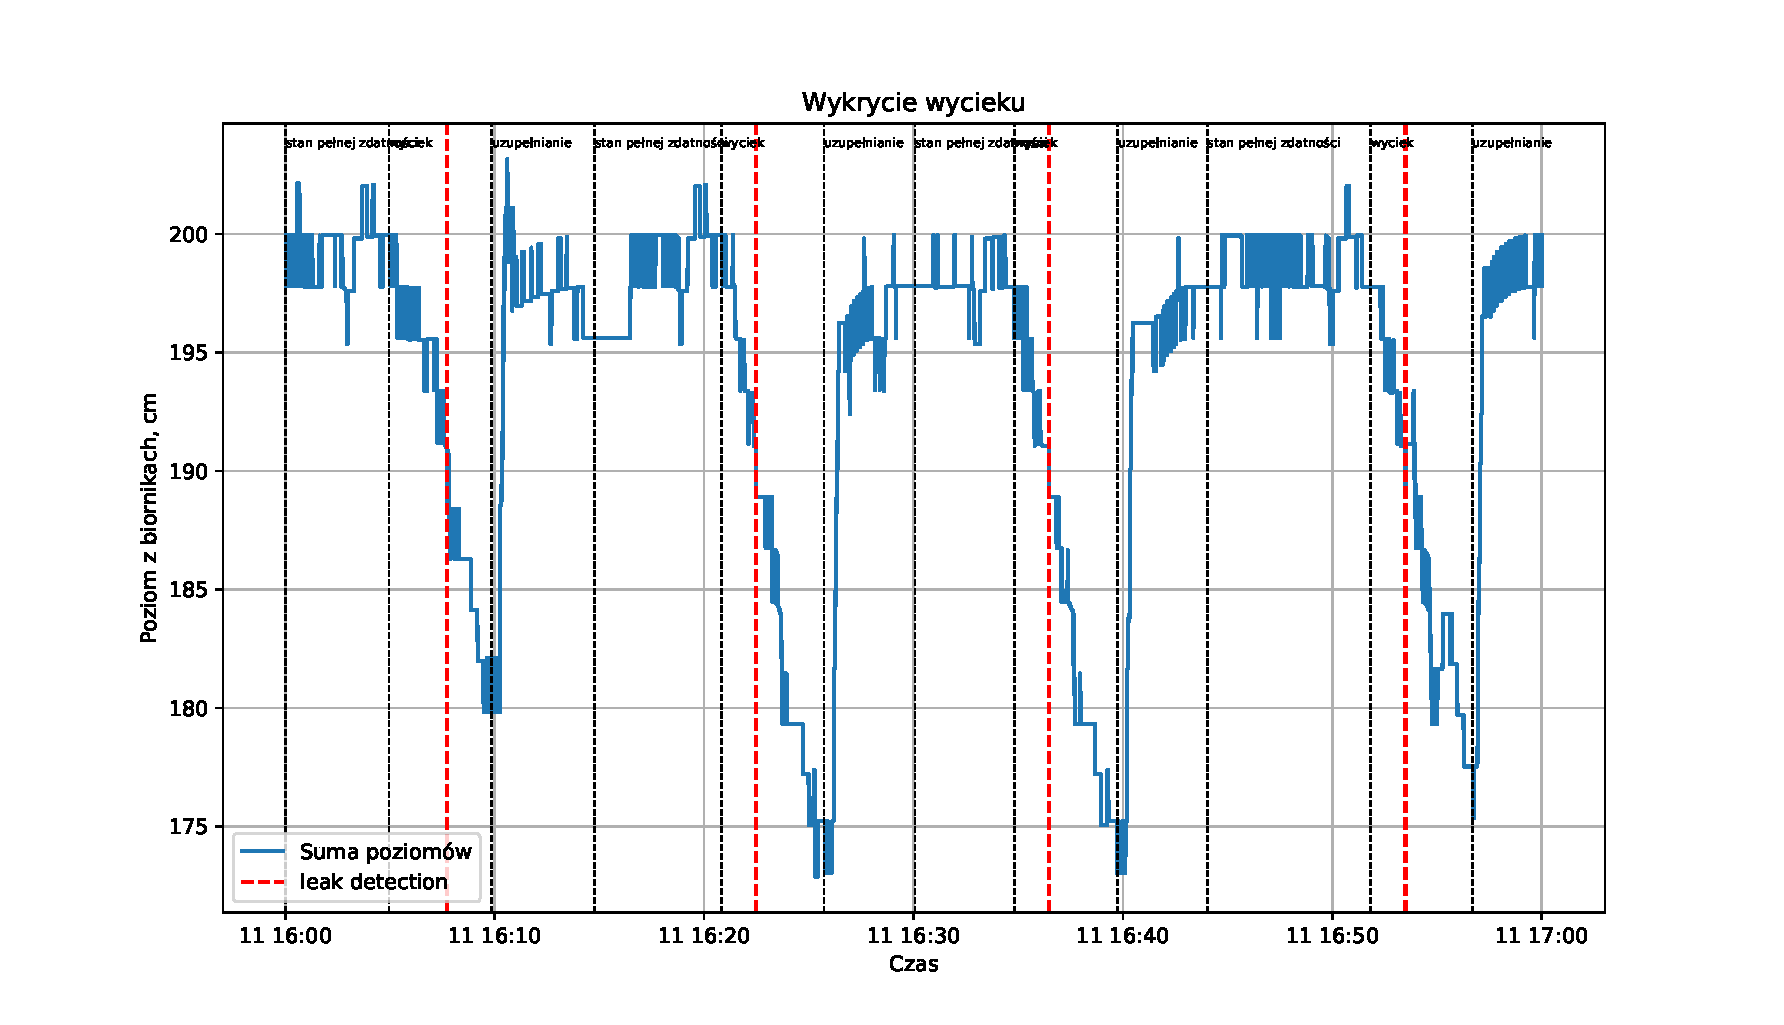
\includegraphics[width=0.8\textwidth]{leak_detection}
        \caption{wykrycie wycieku}
        \label{fig:wyciek1}
\end{figure}

Testy przeprowazdono dla wszystkich przebiegów. Zestawienie przedsatwiono w tabeli \ref{tab:wyciek2}.

\begin{table}[H]
\centering
\caption{Wyniki testu wykrycia wycieku}
\begin{tabular}{lcccc}
\toprule
Zestaw danych & F1\_data & F2\_data & F3\_data & F4\_data\\
\midrule
Rzeczywiste awarie & 0 & 0 & 4 & 0\\
Wykryte awarie & 0 & 0 & 4 & 0\\
\bottomrule
\end{tabular}
\label{tab:wyciek2}
\end{table}

Jak widać wszystkie wycieki zostały skutecznie wykryte, nie wystąpiły również fałszywe alarmy dla żadnego z przebiegów.

\subsection{Wykrycie cyberataku}

W celu wykrycia cyberataku sprawdzane są oscylacje regulowanych wartości ciśnienia. W celu wykrycia oscylacji, wartość mierzona filtrowana jest górnoprzepustowo, a następnie brana jest wartosc bezwględna (w testach dało to lepsze rezultaty niż RMS). Wartość ta następnie jest filtrowana dolnoprzepustowo i porównywana z wybranym progiem. Jeśli poziom utrzymuje się dłużej niż określony czas uznaje się, że wystąpił cyberatak. Wartość progu oraz czasu zostały dobrane arbitralnie. Na rys. \ref{fig:atak1} przedstawiono działanie testu diagnostycznego dla przebiegu z awariami. Jak widać, wszystkie cyberataki zostały wykryte, oraz nie wystąpiły fałszywe alarmy.

\begin{figure}[H]
        \centering
        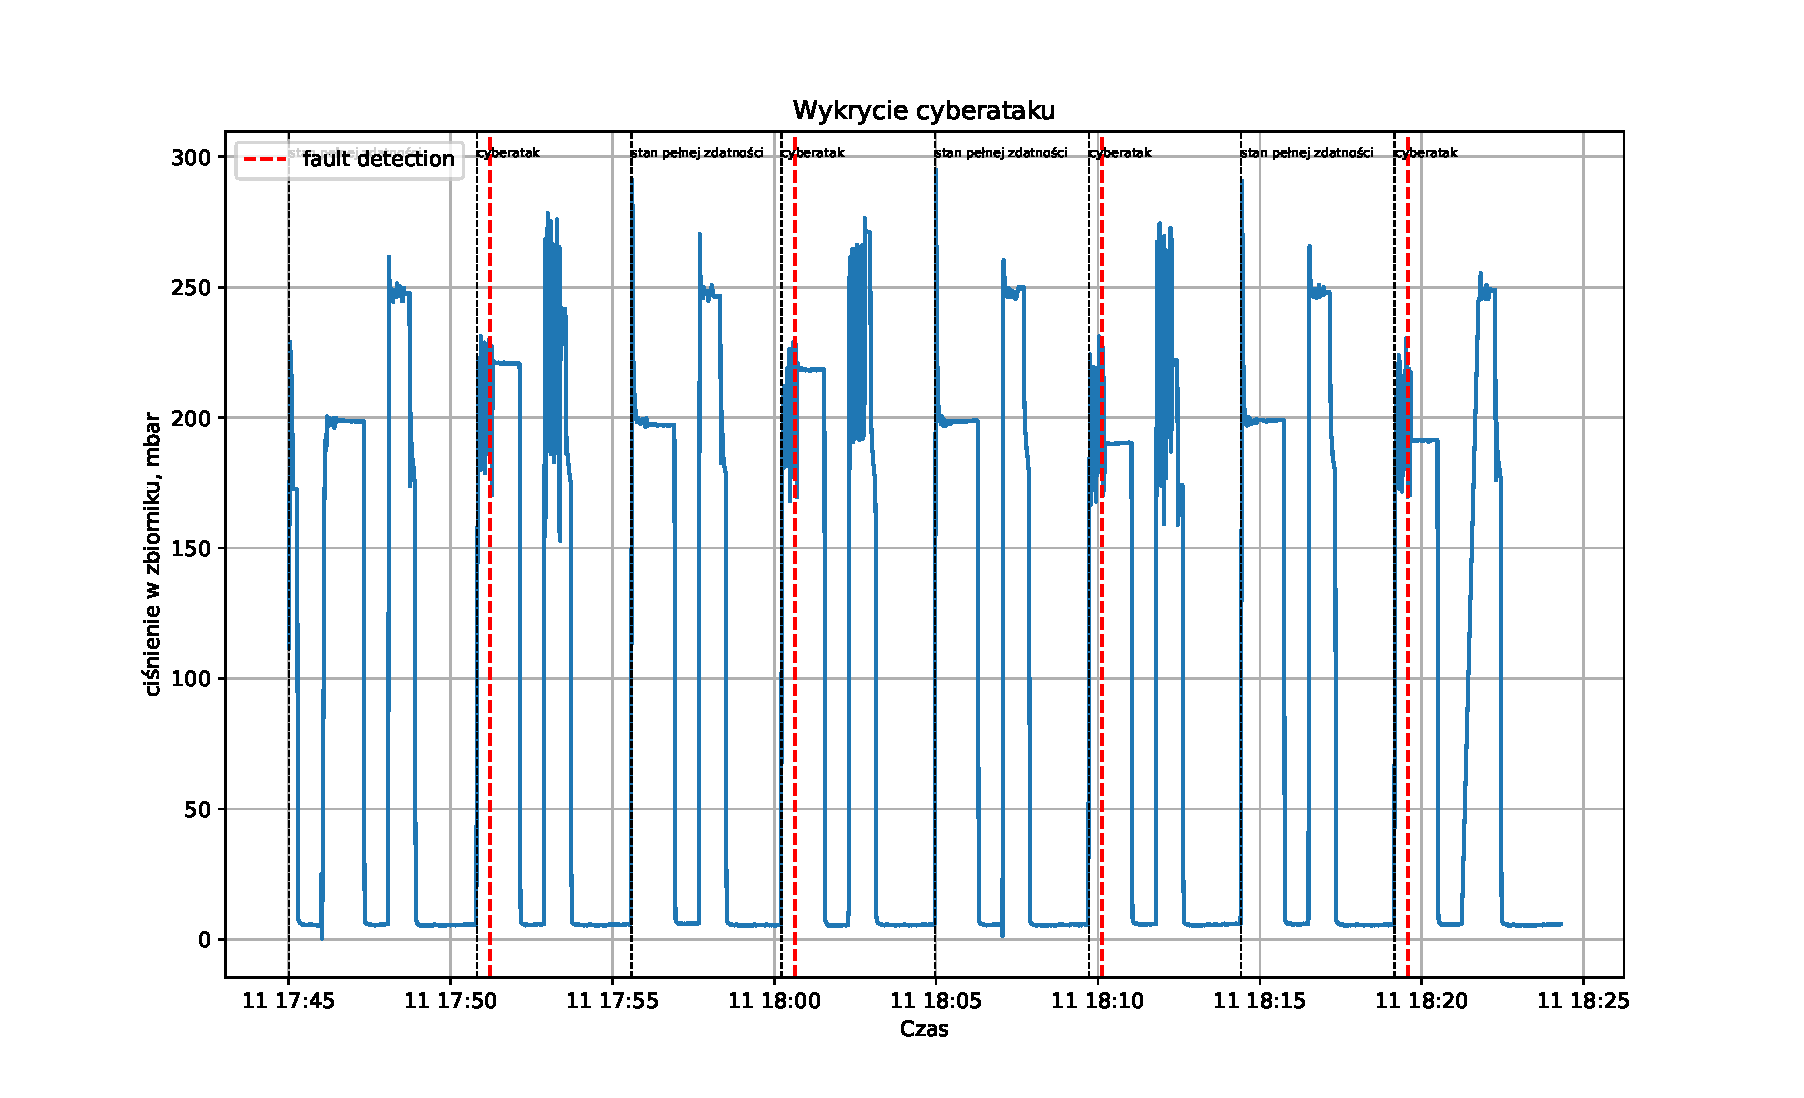
\includegraphics[width=0.8\textwidth]{attack_detection}
        \caption{wykrycie cyberataku}
        \label{fig:atak1}
\end{figure}

Test przeprowadzono dla wszystkich przebiegów. Zestawienie przedstawiono w tabeli \ref{tab:atak2}.

\begin{table}[H]
\centering
\caption{Wyniki testu wykrycia cyberataku}
\begin{tabular}{lcccc}
\toprule
Zestaw danych & F1\_data & F2\_data & F3\_data & F4\_data\\
\midrule
Rzeczywiste awarie & 0 & 4 & 0 & 0\\
Wykryte awarie & 0 & 4 & 0 & 0\\
\bottomrule
\end{tabular}
\label{tab:atak2}
\end{table}

Wszystkie cyberataki zostały skutecznie wykryte, nie wystąpiły również fałszywe alarmy dla żadnego z innych przebiegów.

\subsection{Wykrycie błedu operatora}

Bład operatora jest wykrywany na podstawie różnicy między zadanym ciśnieniem w zbiorniku, a ciśnieniem rzeczywistym. W przypadku błedu operatora ciśnienie w zbiorniku nie jest poprawnie utrzymywane. Jeżeli w fazie, w której ciśnienie w zbiorniku powinno byś utrzymywane, jest ona zbyt niskie przez określony czas, uznaje się, że wystąpił błąd operatora. Wartości progu oraz czasu zostały dobrane arbitralnie. Na rys. \ref{fig:error1} przedstawiono działanie testu diagnostycznego dla przebiegu z awariami. Jak widać, wszystkie błędy operatora zostały wykryte, oraz nie wystąpiły fałszywe alarmy.

\begin{figure}[H]
        \centering
        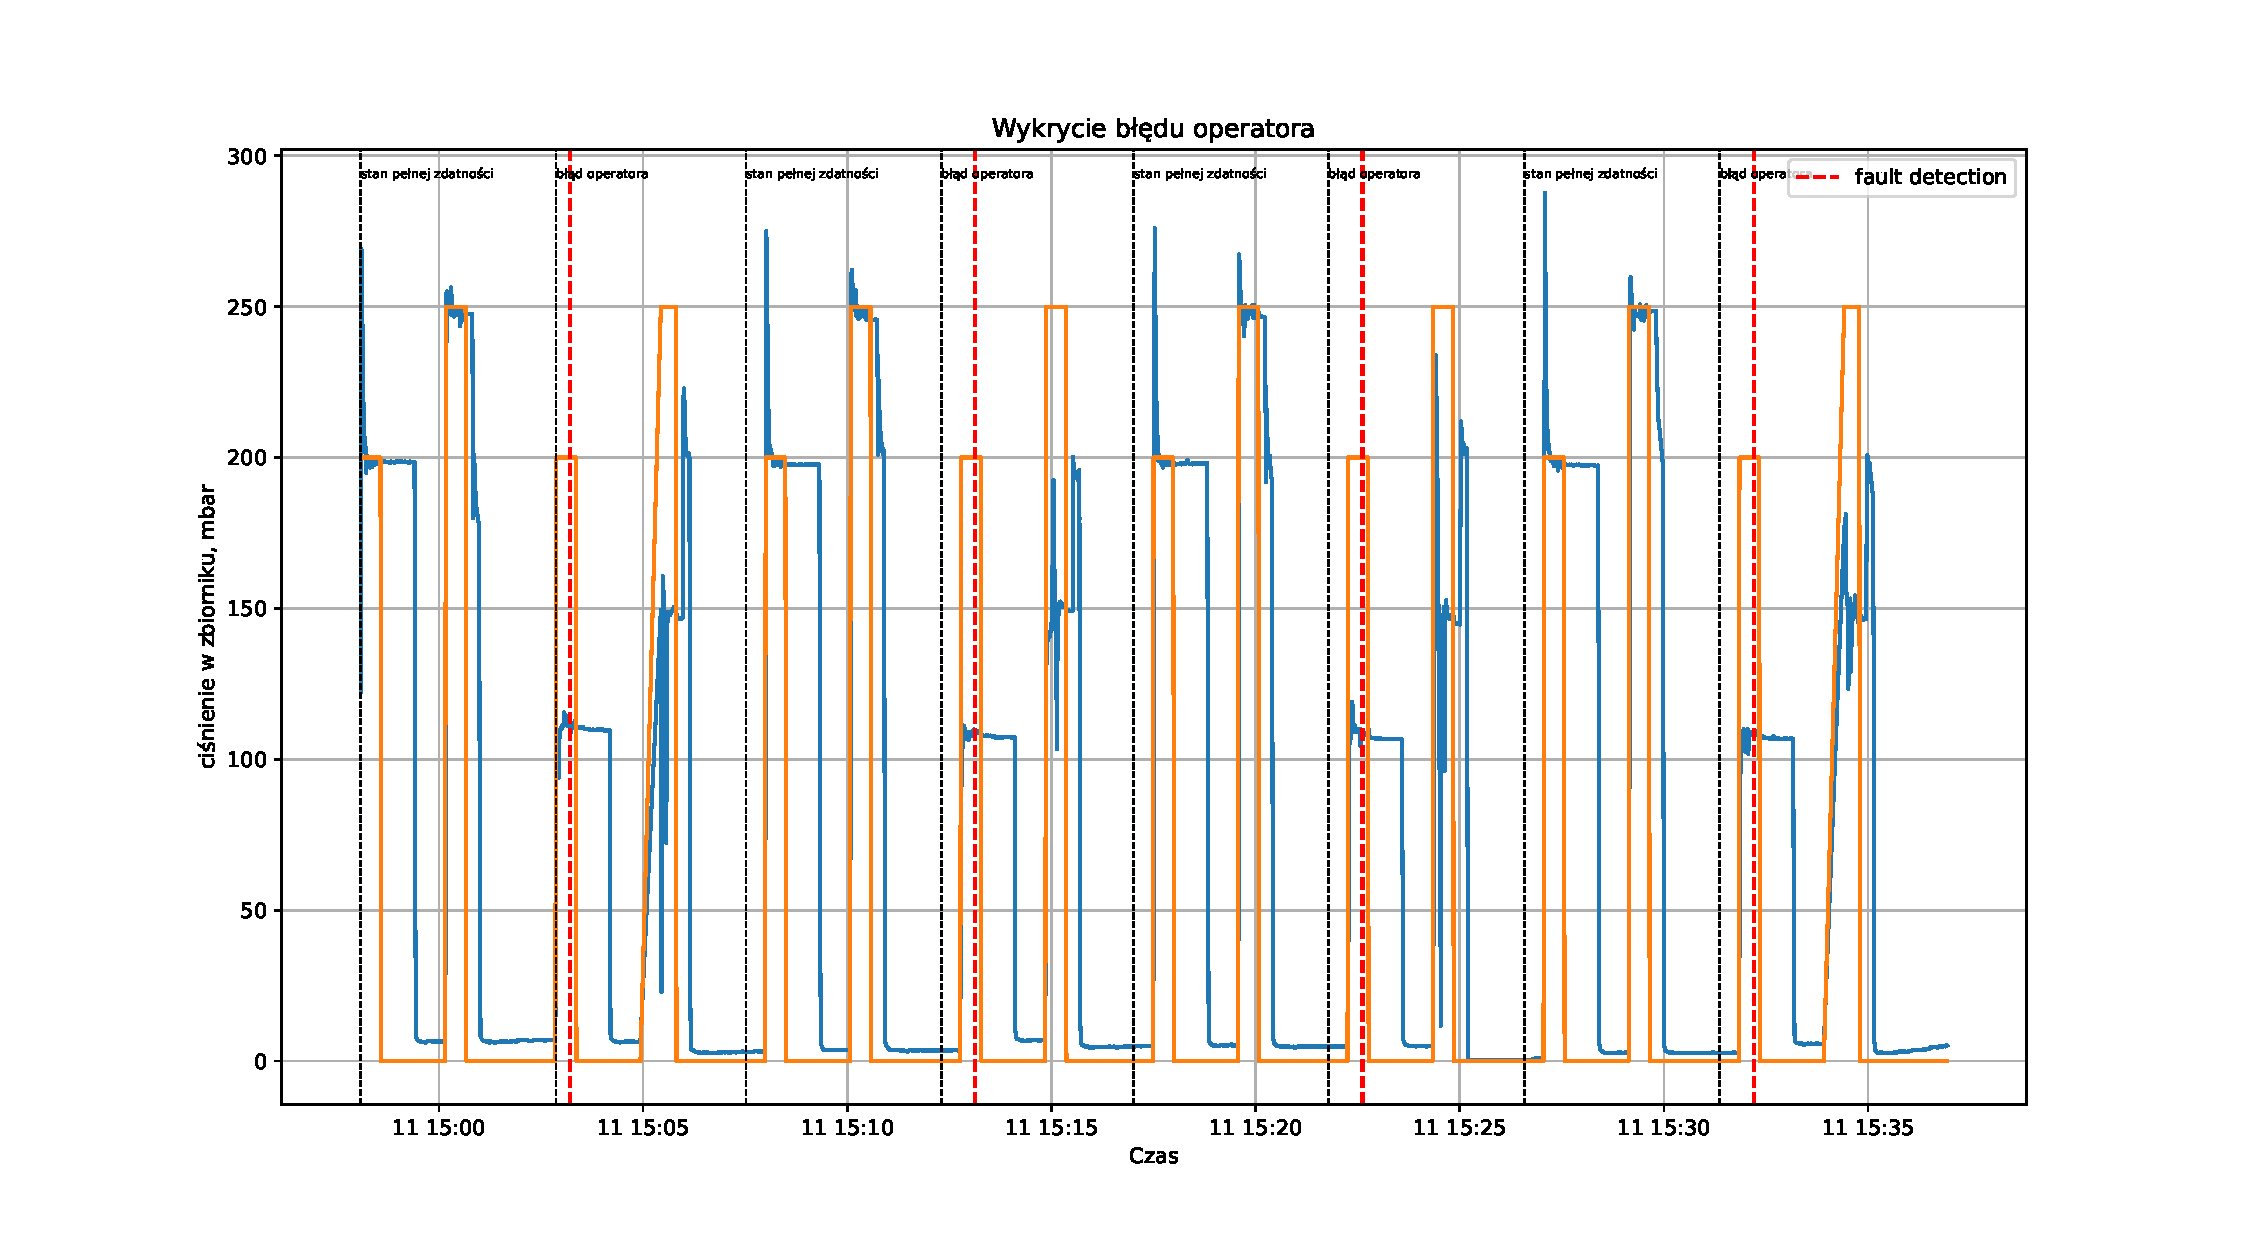
\includegraphics[width=0.8\textwidth]{error_detection}
        \caption{wykrycie błędu operatora}
        \label{fig:error1}
\end{figure}

W tabeli \ref{tab:error2} przedstawiono wyniki testu dla wszystkich przebiegów.

\begin{table}[H]
\centering
\caption{Wyniki testu wykrycia błędu operatora}
\begin{tabular}{lcccc}
\toprule
Zestaw danych & F1\_data & F2\_data & F3\_data & F4\_data\\
\midrule
Rzeczywiste awarie & 0 & 0 & 0 & 4\\
Wykryte awarie & 0 & 1 & 2 & 4\\
\bottomrule
\end{tabular}
\label{tab:error2}
\end{table}

Okazało się, że w przebiegu F2 i F3 (odpowiednio cyberatak i wyciek) zdiagnozowano problemy jako błędy operatora. Oznacza to, zę powyższy sposób nieskutecznie wyizolował problemy

\subsection{Wykrycie przytkania}

W celu wykrycia przytkania sprawdzana jest różnica między zadanym przepływem, a rzeczywistym. W przypadku przytkania, pomimo pełnego wysterowania pompy, nie da się zrealizować rządanego przepływu. Jeżeli przy odpowiednio dużym wysterowaniu przez określony czas utrzymywany jest błąd przepływu uznaje się, że wystąpiło przytkanie. Wartości progu oraz czasu zostały dobrane arbitralnie. Na rys. \ref{fig:zatkanie3} przedstawiono działanie testu diagnostycznego dla przebiegu z awariami.

\begin{figure}[H]
        \centering
        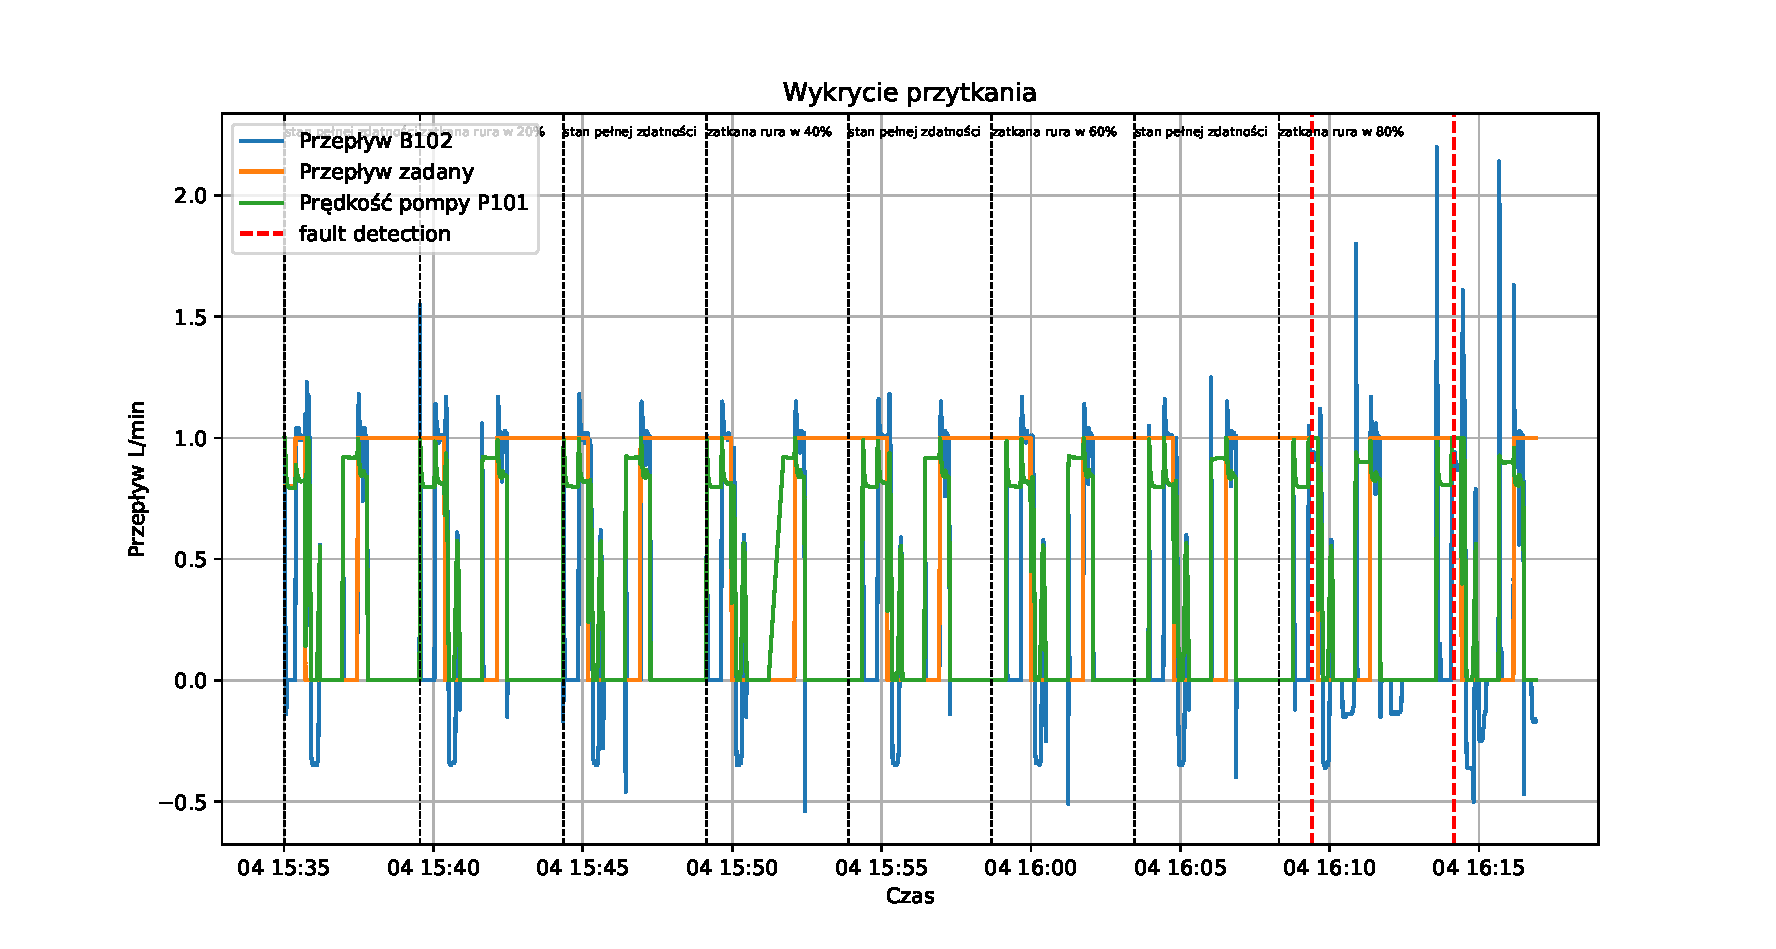
\includegraphics[width=0.8\textwidth]{clogging_detection.pdf}
        \caption{Wykrycie przytkania}
        \label{fig:zatkanie3}
\end{figure}

Jak widać, nie wszystkie przebiegi zostały poprawnie zdiagnozowane.W przypadku małego przytkania pompa skutcznie radziła sobie z zapewnieniem poprawnego przebiegu.

W tabeli \ref{tab:zatkanie2} przedstawiono wyniki testu dla wszystkich przebiegów.

\begin{table}[H]
\centering
\caption{Wyniki testu wykrycia przytkania}
\begin{tabular}{lcccc}
\toprule
Zestaw danych & F1\_data & F2\_data & F3\_data & F4\_data\\
\midrule
Rzeczywiste awarie & 4 & 0 & 0 & 0\\
Wykryte awarie & 2 & 8 & 1 & 8\\
\bottomrule
\end{tabular}
\label{tab:zatkanie2}
\end{table}

Tutaj okazało się, że zaproponowany sposób zgłasza bardzo dużo fałszywych alarmów. Co więcej, dla innych przebiegów awarie były zgłaszane nawet w momentach które powinny być uznane za sprawne. Jednak na prebiegach rzeczywisćie da się zaobserować anormalne zachowanie i niezapewnienie rządanego przzepływu w tych momentach.

\section{Wskaźniki alarmów}

W celu określenia poprawności przedsatwionych algorytmów wykrywania alarmów obliczono wskaźniki dla każdej z metod. Skrypty przerobiono tak, by dla każdej próbki czasowej była określona wartość alarmu. Wyznaczoną wartosć porónano z zadeklarowaną wartością z pliku. Przebiegi sygnałów alarmów przedstawiono na rysunkach \ref{fig:wyciek5} do \ref{fig:zatkanie5}. dodatkowo przyjęto, że usuniecie usterki powodowao wyłączenie alarmu.

\begin{figure}[H]
        \centering
        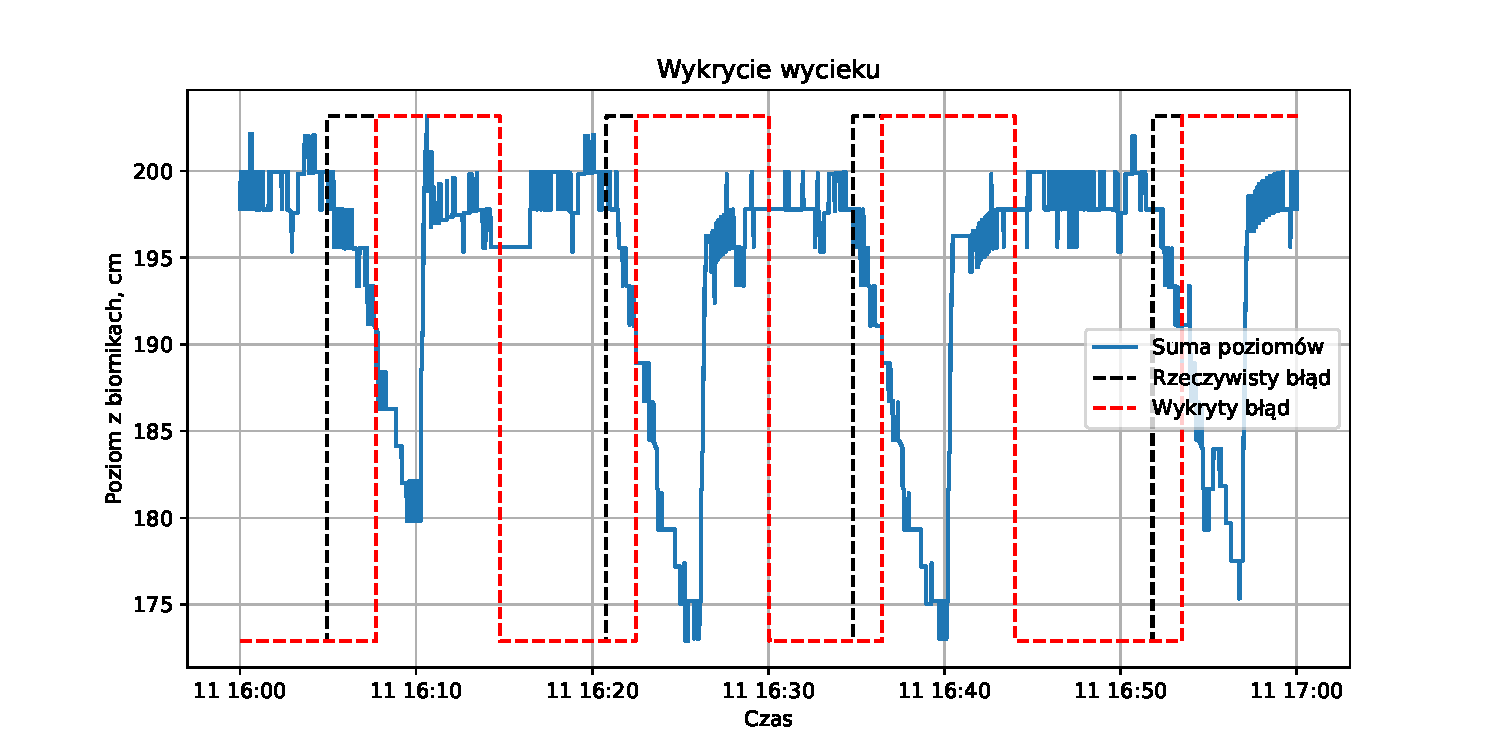
\includegraphics[width=0.8\textwidth]{leak_detection_wskazniki.pdf}
        \caption{Wykrycie wycieku}
        \label{fig:wyciek5}
\end{figure}

\begin{figure}[H]
        \centering
        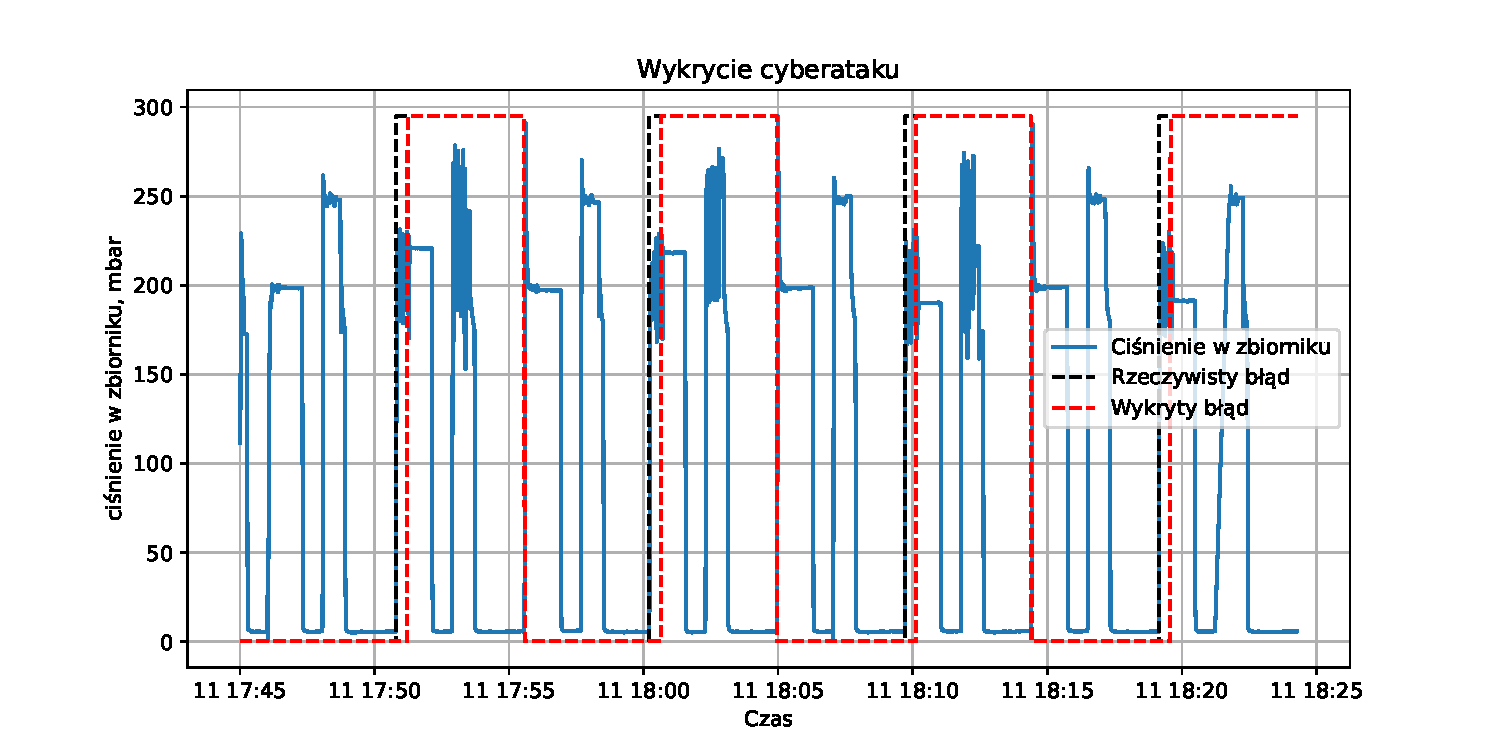
\includegraphics[width=0.8\textwidth]{attack_detection_wskazniki.pdf}
        \caption{Wykrycie cyberataku}
        \label{fig:atak5}
\end{figure}

\begin{figure}[H]
        \centering
        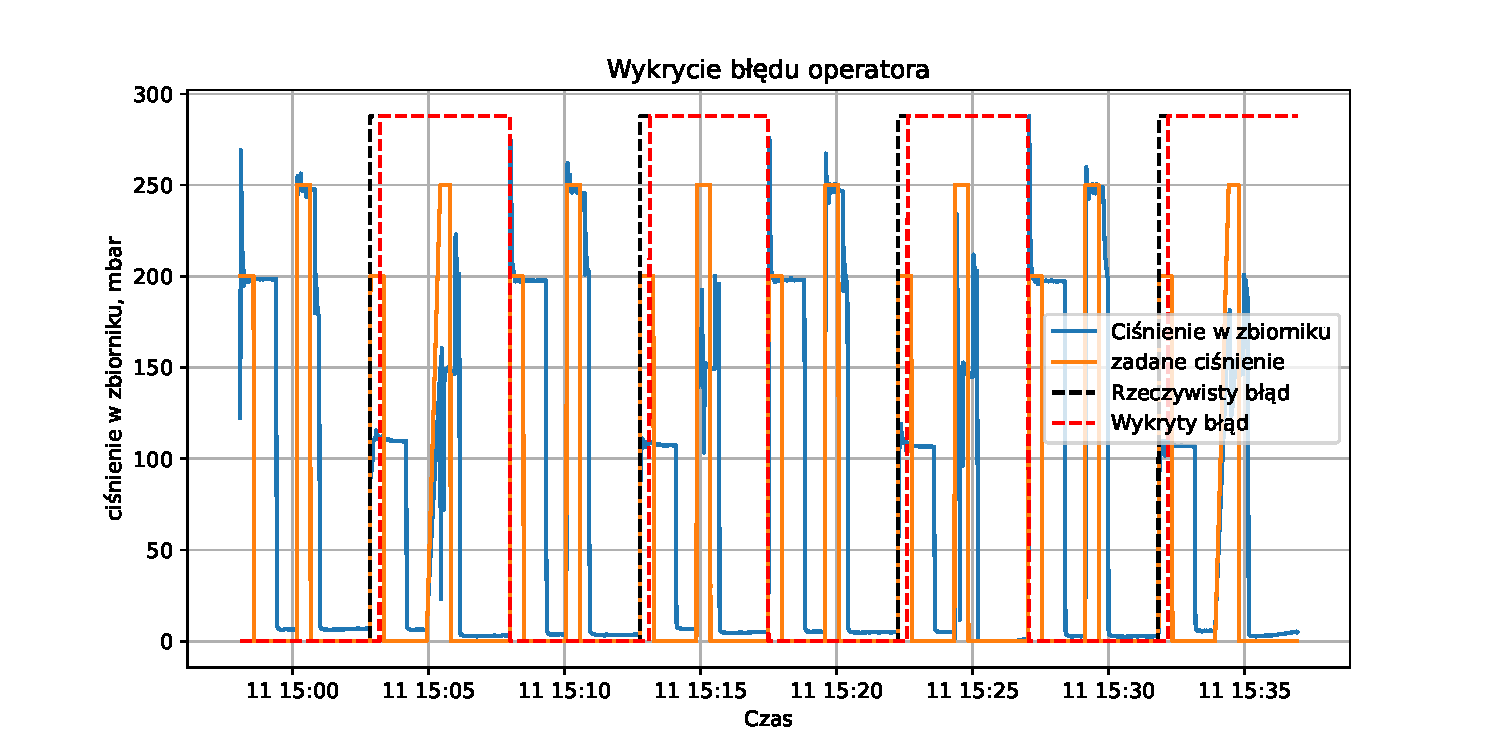
\includegraphics[width=0.8\textwidth]{error_detection_wskazniki.pdf}
        \caption{Wykrycie błędu operatora}
        \label{fig:error5}
\end{figure}

\begin{figure}[H]
        \centering
        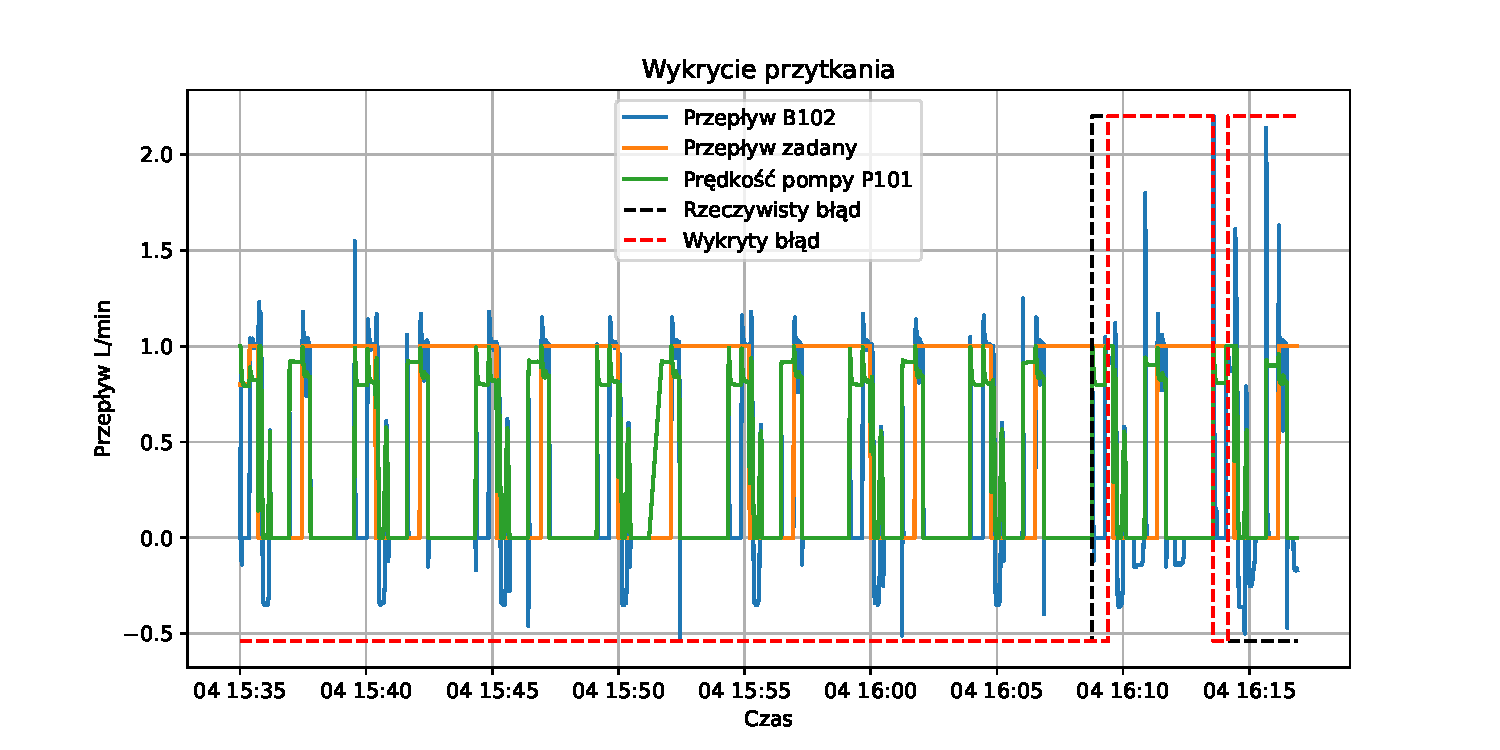
\includegraphics[width=0.8\textwidth]{clogging_detection_wskazniki.pdf}
        \caption{Wykrycie przytkania}
        \label{fig:zatkanie5}
\end{figure}

Na podstawie danych obliczone wskaźniki przedstawiono w tabeli \ref{tab:wskaźniki}. Każdorazowo wyznaczano je dla dedykowanego zestawu danych.

\begin{table}[H]
\centering
\caption{Wskaźniki alarmów}
\begin{tabular}{lcccc}
\toprule
Diagnozowany alarm & \textbf{Wyciek} & \textbf{Cyberatak} & \textbf{Błąd operatora} & \textbf{Przytkanie}\\
\midrule
Wskaźnik fałszywych alarmów & 0 \% & 0 \% & 0 \% & 7,5 \% \\
Wskaźnik prawidłowyc alarmów & 78,7 \% & 91,1 \% & 92,5 \% & 86,8 \% \\
\bottomrule
\end{tabular}
\label{tab:wskaźniki}
\end{table}

Na danych można zaobserować, ze fałszywe alarmy praktycznie nie wystepowały. Jedyny przypadek fałszywego alarmu wystąpił przy przytkaniu, ale na zebranych danych rzeczywiście można zaobserwowac anomalie, co podaje w wątpliwość prawdziwość informacji o stanie układu.

Wszystkie usterki zostały wykryte, zazwyczaj w dość krótkim czasie.


% \subsection{Wykresy sygnałów diagnostycznych}


% \subsection{Wyznaczenie wskaźników detekcji uszkodzeń}

% \section{Testy diagnostyczne bazujące na modelu obiektu}


% \subsection{Wykresy sygnałów diagnostycznych}


% \subsection{Wyznaczenie wskaźników detekcji uszkodzeń}


% \section{Izolacja uszkodzeń}


% \section{Wnioski}


\end{document}
